\documentclass[tikz,border=10pt]{standalone}
\usepackage{tikz}
\usepackage{amsmath,amssymb}
\usetikzlibrary{matrix,arrows,positioning,calc}

\begin{document}
	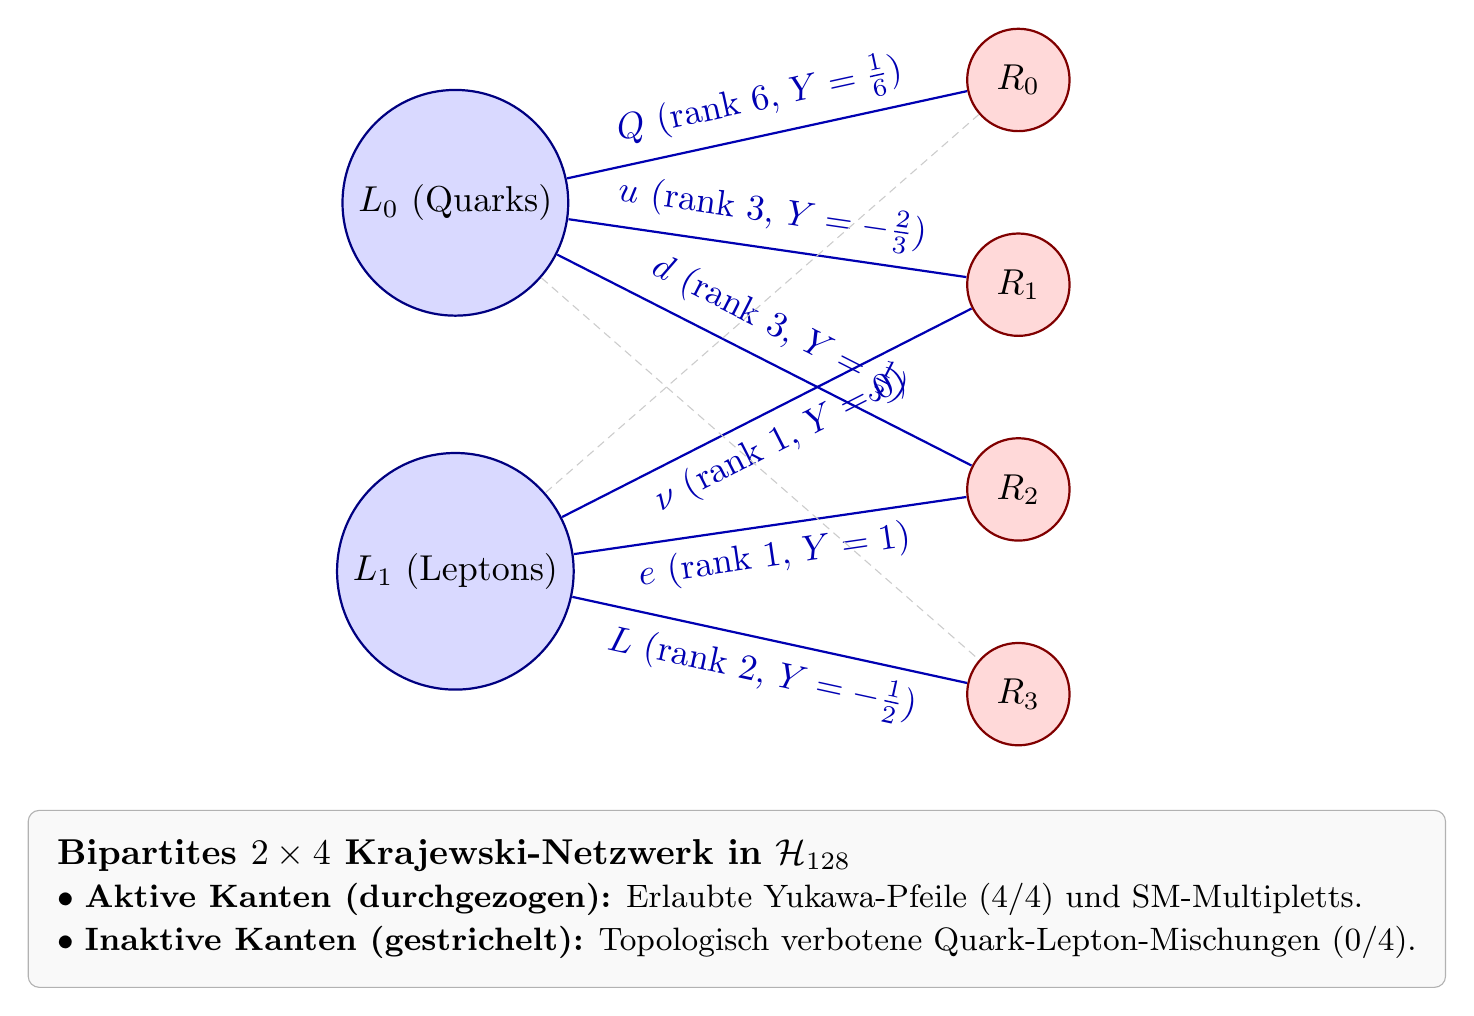
\begin{tikzpicture}[scale=1.3, every node/.style={transform shape}]
		% Styles
		\tikzstyle{leftvertex}=[circle, draw=blue!50!black, fill=blue!15, thick, minimum size=10mm]
		\tikzstyle{rightvertex}=[circle, draw=red!50!black, fill=red!15, thick, minimum size=10mm]
		\tikzstyle{edge}=[thick, blue!70!black]
		\tikzstyle{inactiveedge}=[thin, densely dashed, gray!40]
		
		% Left Vertices (L_0: Quarks, L_1: Leptons)
		\node[leftvertex] (L0) at (0, 1.8) {$L_0$ (Quarks)};
		\node[leftvertex] (L1) at (0, -1.8) {$L_1$ (Leptons)};
		
		% Right Vertices (R_0 to R_3)
		\node[rightvertex] (R0) at (5.5, 3.0) {$R_0$};
		\node[rightvertex] (R1) at (5.5, 1.0) {$R_1$};
		\node[rightvertex] (R2) at (5.5, -1.0) {$R_2$};
		\node[rightvertex] (R3) at (5.5, -3.0) {$R_3$};
		
		% Active Edges (Kanten des physikalischen Modells mit Rängen und Hypercharges)
		\draw[edge] (L0) -- node[above, sloped] {$Q$ (rank 6, $Y=\frac{1}{6}$)} (R0);
		\draw[edge] (L0) -- node[above, sloped] {$u$ (rank 3, $Y=-\frac{2}{3}$)} (R1);
		\draw[edge] (L0) -- node[above, sloped] {$d$ (rank 3, $Y=\frac{1}{3}$)} (R2);
		
		\draw[edge] (L1) -- node[below, sloped] {$\nu$ (rank 1, $Y=0$)} (R1);
		\draw[edge] (L1) -- node[below, sloped] {$e$ (rank 1, $Y=1$)} (R2);
		\draw[edge] (L1) -- node[below, sloped] {$L$ (rank 2, $Y=-\frac{1}{2}$)} (R3);
		
		% Inactive / Empty Cells (Kanten mit Null-Kopplung / topologischer Schutz)
		\draw[inactiveedge] (L0) -- (R3);
		\draw[inactiveedge] (L1) -- (R0);
		
		% Legend / Box
		\node[draw=black!30, rounded corners, inner sep=8pt, fill=gray!5, align=left] at (2.75, -5.0) {
			\textbf{Bipartites $2 \times 4$ Krajewski-Netzwerk in $\mathcal{H}_{128}$}\\
			{\small $\bullet$ \textbf{Aktive Kanten (durchgezogen):} Erlaubte Yukawa-Pfeile ($4/4$) und SM-Multipletts.}\\
			{\small $\bullet$ \textbf{Inaktive Kanten (gestrichelt):} Topologisch verbotene Quark-Lepton-Mischungen ($0/4$).}
		};
	\end{tikzpicture}
\end{document}